%%%%%%%%%%%%%%%%%%%%%%%%%%%%%%%%%%%%%%%%%% 9 - 1
\section{Измерение массы плоской фигуры}
%\LabTheme{Центр масс. Правило рычага}
\LabHeader{предложить способ измерения массы плоской фигуры неправильной формы, исключающий её взвешивания на весах.}{плоская фигура, линейка, гирька, стол.}
\SolveVariant
\begin{enumerate}
\item Найдём центр масс плоской фигуры. Для этого фигуру можно положить на стол так, чтобы она опиралась только на край стола, и провести по ней карандашом линию вдоль края стола. Затем эту операцию надо повторить, изменив положение фигуры на столе. Центр масс будет находится в точке пересечения этих двух прямых линий.\par
\begin{figure}[h]
  \parbox[b]{0.49\textwidth}{
    \centering
    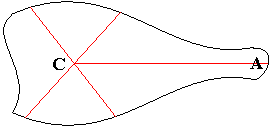
\includegraphics{9kl1-1.png}
    \caption{Центр масс}
  }
  \hfil
  \parbox[b]{0.49\textwidth}{
    \centering
    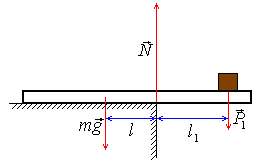
\includegraphics{9kl1-2.png}
    \caption{Равенство моментов}
    \label{fig:9kl1:moments}
  }
\end{figure}
\item Проведём на фигуре линию в произвольном направлении от центра масс (линия \( AC \)). Положим гирю на линию \( AC \) недалеко от края фигуры и, используя край стола как точку опоры, сбалансируем рычаг (рис.~\ref{fig:9kl1:moments}). Записывая условие равенства моментов сил, приложенных к фигуре, получаем \( m=\frac{l_1}{l} m_\text{гири} \).
\end{enumerate}
\MesErrors
Погрешность определения массы вычисляется по формуле:
\begin{equation*}
\varepsilon m = \frac{\Delta m_\text{гири}}{m_\text{гири}} + \frac{\Delta l_1}{l_1} + \frac{\Delta l}{l}=\frac{\Delta m_\text{гири}}{m_\text{гири}} + \Delta l\left( \frac{1}{l_1} + \frac{1}{l}\right)
\end{equation*}
\SchoolBase
\begin{itemize}
  \item Определение центра масс.
  \item Правило рычага. Определение момента силы.
\end{itemize}
\AdditionalQuestions
\begin{itemize}
  \item Применим ли метод, если край стола не будет перпендикулярен  \( AC \)? Почему?\par
    \Answer да, применим. При этом плечи сил тяжести фигуры и гири будут проходить перпендикулярно к краю стола под некоторым углом к \( AC \), но их отношение будет таким же, как отношение частей отрезка \( AC \), на которые его делит край стола.
\end{itemize}
%%%%%%%%%%%%%%%%%%%%%%%%%%%%%%%%%%%%%%%%%% 9 - 2
\section{Определение плотности пластелина}
\LabHeader{определить плотность куска пластелина, считая плотность воды известной.}{кусок пластилина, линейка, сосуд цилиндрической формы с водой.}
\SolveVariant
Для нахождения плотности пластелина \(\rho\) удобно испльзовать <<кораблик>>:
\begin{enumerate}
  \item Опустим кусок пластелина в воду, определим высоту подъема уровня воды \(\Delta h_1\). Тогда объем пластелина будет \(V=S\Delta h_1\), где \(S\) "--- площадь сечения сосуда.
  \begin{figure}[h]
    \centering
    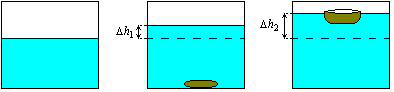
\includegraphics[width=\textwidth]{9kl2-1.png}
    \caption{Метод <<кораблика>>}
  \end{figure}
  \item Изготовим из пластелина <<кораблик>>, опустим его на воду. Измерим высоту подъема уровня воды \(\Delta h_2\) в этом случае. Масса вытесненной воды будет \(m=\rho_\text{воды} S\Delta h_2 \), что равно массе кораблика. Отсюда получаем, что \( \rho = \rho_0 \frac{\Delta h_2}{\Delta h_1}\)
\end{enumerate}
\MesErrors
Погрешность определения вычисляется по формуле:
\begin{equation*}
\varepsilon \rho = \frac{\Delta(\Delta h_1)}{\Delta h_1} + \frac{\Delta(\Delta h_2)}{\Delta h_2}=\Delta(\Delta h) \left( \frac{1}{\Delta h_1} + \frac{1}{\Delta h_2} \right)
\end{equation*}
\SchoolBase
\begin{itemize}
  \item Закон Архимеда. Условие плавания тел.
\end{itemize}
\AdditionalQuestions
\begin{itemize}
  \item Почему справедлива формула \(V_\text{вытесненной воды} = S\Delta h\), где \(\Delta h\) "--- изменение уровня воды при спуске плавающего тела на воду, \(S\) "--- площадь сосуда?\par
   % \begin{floatingfigure}[rflt]{0.4\textwidth}
  \begin{figure}[h!]
    \centering
    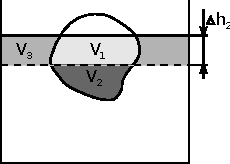
\includegraphics[width=0.4\textwidth]{9kl2-2.pdf}
    \caption{Объем вытесняемой воды}
    \label{fig:9kl2:vol}
 % \end{floatingfigure}
 \end{figure}
  \Answer чтобы это объяснить, удобно нарисовать тело неправильной формы, плавающее в воде, и на этом же рисунке изобразить уровень воды в отсутствие тела (на рис.~\ref{fig:9kl2:vol} изображен пунктиром). \label{ans:9kl2:vol}
 При этом объем погруженой части \(V_\text{п} = V_1 + V_2\). Поскольку объем воды постоянен, \(V_2 = V_3\) (вода как-бы перешла из \(V_2\) в \(V_3\) при погружении тела), видно, что \(V_\text{п} = V_1 + V_2=V_1+V_3=S\Delta h_2\).
  \item Чем может быть обусловлена большая погрешность измерений? Что можно предпринять для увеличения точности определения плотности пластелина?\par
  \Answer Она обычловлена большой площадью сосуда, вследствие чего изменение уровня воды "--- мало по сравнению с погрешностью измерения длины. Для уменьшения погрешности можно взять другой сосуд меньшей площади, либо увеличить количество пластелина.
\end{itemize}
%%%%%%%%%%%%%%%%%%%%%%%%%%%%%%%%%%%%%%%%%% 9 - 3
\section{Определение плотности неизвестного металла}
\LabHeader{найти плотность кусочков неизвестного металла и определить, какой металл был дан, руководствуясь таблицей плотностей.}{сосуд цилиндрической формы с водой, стакан, плавающий в нём, мелкие кусочки металла, линейка}
\SolveVariant
\begin{enumerate}
  \item Определим массу стакана \(m_\text{ст}\). Для этого опустим его свободно плавать. После этого измерим изменение уровня воды \(\Delta h_1\) при этом. Тогда, по закону Архимеда, масса стакана будет: \(m_\text{ст} = \rho_0 \Delta h_1 S\), где \( \rho_0 \) "--- плотность воды, \(S\) "--- площадь сечения сосуда.
  \item Определим массу кусочков неизвестного металла \(m_\text{мет}\). Опустим их в плавающий стакан. Измерим изменение уровня воды \(\Delta h_2\). По закону Архимеда, общая масса стакана и кусочков металла будет: \(m_\text{ст} + m_\text{мет} = \rho_0 \Delta h_2 S\). Тогда имеем: \( m_\text{мет} = \rho_0 (\Delta h_2 - \Delta h_1) S\).
  \item Определим объем кусочков металла \(V_\text{мет}\). Для этого погрузим их в воду. То \(V_\text{мет}=\Delta h_3 S\), где \(\Delta h_3\) "--- изменение уровня воды в этом случае.\par
  Тогда плотность металла будет, по определению, \(\rho = \frac{m_\text{мет}}{V_\text{мет}} = \rho_0 \frac{\Delta h_2 - \Delta h_1}{\Delta h_3}\)
\end{enumerate}
\MesErrors
Погрешность определения плотности выражается по формуле:
\begin{equation*}
\varepsilon \rho = \frac{\Delta(\Delta h_1)+\Delta(\Delta h_2)}{\Delta h_1 - \Delta h_2} + \frac{\Delta(\Delta h_1)}{\Delta h_1}= \Delta(\Delta h) \left(\frac{2}{\Delta h_1 - \Delta h_2} + \frac{1}{\Delta h_1} \right)
\end{equation*}
\SchoolBase
\begin{itemize}
  \item Закон Архимеда. Условие плавания тел.
\end{itemize}
\AdditionalQuestions
\begin{itemize}
  \item Почему справедлива формула \(V_\text{вытесненной воды} = S\Delta h\), где \(\Delta h\) "--- изменение уровня воды при спуске плавающего тела на воду, \(S\) "--- площадь сосуда?\par
  \Answer см. стр. \pageref{ans:9kl2:vol}.
  \item Чем может быть обусловлена большая погрешность измерений? Что можно предпринять для увеличения точности определения плотности кусочков металла?\par
  \Answer Она обусловлена большой площадью сосуда, вследствие чего изменение уровня воды мало по сравнению с погрешностью измерения длины, что особенно сказывается при измерении объема кусочков металла. Для уменьшения погрешности можно взять другой сосуд меньшей площади, либо увеличить количество металла.
\end{itemize}
\AdditionalNotes
\begin{itemize}
  \item Если в качестве стакана используется пластиковый стаканчик, при измерении его массы следует заметить, что она "--- много меньше массы кусочков металла. Её измерение "--- проблематично в принципе, поскольку изменение уровня воды при этом практически отсутствует. Поэтому, массой такого стаканчика следует пренебречь, и использовать формулу \(\rho \approx \rho_0 \frac{\Delta h_2}{\Delta h_3}\).
\end{itemize}
%%%%%%%%%%%%%%%%%%%%%%%%%%%%%%%%%%%%%%%%%% 9 - 4
\section{Определение массы легкого груза}
\LabHeader{определить массу бруска.}{брусок, штатив, нить, угольник, динамометр с большой ценой деления, не позволяющей взвесить брусок непосредственно.}
\SolveVariant
Для измерения следует собрать установку, изображенную на рис.~\ref{fig:9kl4:inst}. Записывая условие равновесия системы из второго закона Ньютона, получаем:
\begin{equation*}
    \begin{cases}
    mg=N\cos\alpha\\
    F=N\sin\alpha
    \end{cases}
    \Rightarrow m=\frac{F}{g} \ctg \alpha = \frac{F h}{g x}
\end{equation*}
Измерения следует повторить несколько раз для разных углов \(\alpha\). Удобно закрепить отвес в точке крепления нити, держащей груз, для облегчения измерения \(h\). Для точной горизонтальной ориентиции динамометра удоно использовать угольник.
\begin{figure}[h]
    \centering
    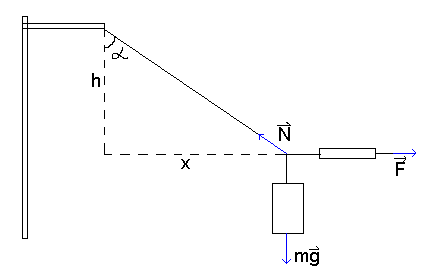
\includegraphics[width=0.4\textwidth]{9kl4-1.png}
    \caption{Установка для измерения массы бруска}
    \label{fig:9kl4:inst}
 \end{figure}
\MesErrors
Погрешность определения массы при каждом конкретном измерении определяется формулой:
\begin{equation}
    \varepsilon m = \frac{\Delta F}{F} + \frac{\Delta h}{h} + \frac{\Delta x}{x}= \frac{\Delta F}{F}+\Delta h \left(\frac{1}{h} + \frac{1}{x}\right)
    \label{eq:9kl4:err}
\end{equation}
\SchoolBase
\begin{itemize}
    \item Векторные физические величины. Вектор силы.
    \item Второй закон Ньютона. Условие равновесия тела.
\end{itemize}
\AdditionalQuestions
\begin{itemize}
    \item Влияет ли неидеальность нити на результат измерений?\par
    \Answer нет, не влияет. Идеальность нити не используется в выведении формулы \(m=\frac{F h}{g x}\). Влияние будет только в случае значительного провисания, но в реальных условиях для этого нужна очень тяжелая нить.
    \item Качественно объяснить, какие значения может принимать угол \(\alpha\), чтобы точность измерений была высокой?\par
    \Answer угол не должен быть близким к~0\textdegree и к~90\textdegree. Иначе либо \(h\), либо \(x\) принимает слишком маленькое для измерения значение, и в формуле для определения погрешности члены \(\frac{\Delta h}{h}\) или \(\frac{\Delta x}{x}\) становятся слишком большими.
   % \Answer ПустьОценить границы изменения угла можно оценить так:
   \item \textit{(требует представления о тригонометрии)} В каких пределах может изменяться угол \(\alpha\) при погрешности определения массы не более \(\xi=10\% \)? Погрешность измерения силы считать равной нулю.\par
   \Answer Для оценки можно считать, что в формуле~\eqref{eq:9kl4:err} выполняется ограничение \(\frac{\Delta h}{h} \leq \frac{\xi}{2}\) и \(\frac{\Delta h}{x} \leq \frac{\xi}{2}\):
   \begin{equation*}
    \begin{array}{@{}l@{}}
        \begin{cases}
            \frac{\Delta h}{h} \leq \frac{\xi}{2} \\
            \frac{\Delta h}{x} \leq \frac{\xi}{2}
        \end{cases}\\
        l=\sqrt{x^2+h^2}
    \end{array}
    \Rightarrow
    \begin{array}{@{}l@{}} 
    	\cos \alpha = \frac{h}{l} \geq \frac{2\Delta h}{l\xi} \\
    	\sin \alpha = \frac{x}{l} \geq \frac{2\Delta h}{l\xi}
    \end{array}
    \end{equation*}
    При этом, если \(\frac{2\Delta h}{l\xi}>\cos45\text{\textdegree}=\sin45\text{\textdegree}=\frac{\sqrt{2}}{2}\), требуемую точность достичь невозможно.
\end{itemize}
%%%%%%%%%%%%%%%%%%%%%%%%%%%%%%%%%%%%%%%%%% 9 - 5
\section{Исследование неидеального источника наряжения}
\LabHeader{получить зависимость тока в цепи и напряжения на нагрузке от её сопротивления. Постараться объяснить полученный результат.}{источник постоянного тока, реостат, вольтметр, амперметр, соединительные провода.}
\SolveVariant
%\begin{circuit}0
%    \npn1 {Tr-r} B 1
%\end{circuit}
\begin{enumerate}
    \item Для проведения требуемых измерений соберём схему, изображенную на рис.~\ref{fig:9kl5:sch}.
    \begin{figure}[h]
        \centering
        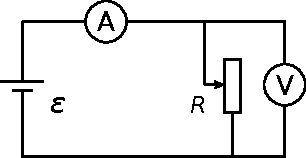
\includegraphics[width=0.4\textwidth]{9kl5-1.pdf}
        \caption{Схема установки}
        \label{fig:9kl5:sch}
    \end{figure}
    \item Изменяя сопротивление реостата, снимем зависимость тока через реостат от напряжения на нём.
    \item Для каждого измерения вычислим сопротивление реостата по закону Ома: \(R_i=\frac{U_i}{I_i}\). Построим искомые графики: \(U(R)\) и \(I(R)\). Желательно отметить прямоугольники ошибок на графике.
\end{enumerate}
\MesErrors
Для определения погрешности сопротивления используется формула: \(\varepsilon R_i=\frac{\Delta I}{I_i}+\frac{\Delta U}{U_i}\). Учитывая, что для цифровых мультиметров погрешность считается как:
\begin{equation*}
    \Delta I = I\varepsilon I_\text{инстр} + \Delta I_\text{суб}
    \Delta U = U\varepsilon U_\text{инстр} + \Delta U_\text{суб}
\end{equation*}
    где ведичины с индексом <<инстр>> "--- заданные относительные инструментальные погрешности приборов, а с индексом <<суб>> "--- субъективные погрешности, равные половине цены деления соотвествтвующего прибора (название <<субъективные>> здесь не совсем логично).
    Тогда \( \varepsilon R_i = \varepsilon I_\text{инстр}+\frac{\Delta I_\text{суб}}{I_i}+\varepsilon U_\text{инстр} +\frac{\Delta U_\text{суб}}{U_i} \), \(\Delta R_i = R_i\varepsilon R \).
\SchoolBase
\begin{itemize}
    \item Закон Ома.
    \item Источник ЭДС. Неидеальный источник напряжения.
    \item \textit{(дополнительно)} Закон Джоуля-Ленца. КПД цепи.
\end{itemize}
\AdditionalQuestions
\begin{itemize}
    \item Объяснить поведение графиков \(U(R)\) и \(I(R)\).\par
    \Answer причина <<необычного>> поведения - внутреннее сопротивление источника ЭДС. При этом \(U=\frac{R}{R+r}E\), \(I=\frac{E}{R+r}\), где \(E\) "--- ЭДС источника, а \(r\) "--- его внутреннее сопротивление.
    \item Построить график зависимости КПД цепи \(\eta\) от сопротивления нагрузки:
    \begin{itemize} 
        \item Теоретический (исходя из определенных значений ЭДС и внутреннего сопротивления источника).
        \item Экспериментальный, по определению КПД (\(\eta=\frac{P_\text{полезная}}{P_\text{источника}}\)) по результатам измерений тока и напряжения в каждой точке. При каком сопротивлении на нагрузке выделяется максимальная мощность?
    \end{itemize}
    \Answer \begin{itemize}
        \item Теоретически КПД цепи определяется формулой \(\eta=\frac{R}{R+r}\), Внутреннее сопротивление и ЭДС находится по двум удаленым друг от друга точкам графика \(U(R)\) (или \(I(R)\));
        \item Экспериментально КПД для каждой точке считается как \(\eta=\frac{I^2 R}{IE}=\frac{IR}{E}\).
    \end{itemize}
\end{itemize}
%%%%%%%%%%%%%%%%%%%%%%%%%%%%%%%%%%%%%%%%%% 9 - 6
\section{Оценка механической мощности человека}
\LabHeader{определить мощность, развиваемую человеком при подъеме по лестнице бегом и шагом.}{линейка, секундомер.}
\SolveVariant
\begin{enumerate}
    \item Измерим среднюю высоту одной ступеньки \(h\). Для этого измерим высоту \(k \simeq 4\) ступенек \(h_k\). В результате, \(h=\frac{h_k}{k}\).
    \item Измерим количество ступенек \(n\). Определим высоту всей лестницы: \(H=nh\).
    \item Измерим секундомером время подъема человека по лестнице шагом \(t_\text{ш}\) и бегом \(t_\text{б}\). Тогда совершаемая работа есть \(A=mgH\), где \(m\) "--- масса человека. Соответственно мощность будет \(P_\text{ш} = \frac{mgH}{t_\text{ш}}\); \(P_\text{б} = \frac{mgH}{t_\text{б}}\).
    \item Желательно провести измерения для нескольких разных людей, и определить среднее значение.
\end{enumerate}
\MesErrors
Погрешность определения мощности вычисляется по формуле:
\begin{equation}
    \varepsilon \Delta P_i = \frac{\Delta m}{m} + \frac{\Delta h_k}{h_k} + \frac{\Delta t}{t_i}
\end{equation}
при этом следует уделить внимание ведичине \(\Delta m\): она должна учитывать естественные суточные колебания массы человеческого тела (приемы пищи) "--- составляет примерно 2 кг и погрешность определения массы весами. Также логично ввести дополнительную поправку, если экспериментатор взвешивался значительное время назад.\par
Следует заметить, что эксперимент в принципе имеет оценочную точность, поскольку понятия <<шагом>> и <<бегом>> являются относительными, и у разных людей разная способность к бегу вверх по лестнице.
\SchoolBase
\begin{itemize}
    \item Механические работа и мощность.
\end{itemize}
\AdditionalQuestions
\begin{itemize}
    \item Энергетическая потребность человека составляет примерно 2500 килокалорий в день. Этой энергии хватило бы на подъём человека массой 75 килограмм на высоту 3300 м, что равносильно подъему на 2,3 м в минуту. Очевидно, что такой работы человек не совершает. Куда теряется потредляемая с пищей энергия?\par
    \Answer На поддержание температуры тела и на работу внутренних органов (например, переваривание пищи)
\end{itemize}
\AdditionalNotes
Лестница двухэтажного корпуса ЛФМШи, ведущая к <<пионерке>>, имеет посередине горизонтальный участок. При этом к погрешности измерения времени \(\Delta t\) целесообразно добавить характерное время, за которое человек преодолевает этот участок.
%%%%%%%%%%%%%%%%%%%%%%%%%%%%%%%%%%%%%%%%%% 9 - 7
\section{Определение числа Пи методом Монте-Карло}
\LabHeader{определить приближенно значение числа \(\pi\) методом Монте-Карло.}{линейка, циркуль, два листа бумаги, несколько небольших тяжелых предметов (гайки, шарики или прочие), копировальная бумага.}
\SolveVariant
Суть метода Монте-Карло заключается в следующем: на некоторую область плоскости площадью \(S\) ставится множество равномерно распределенных по координатам точек. При этом вероятность \(p\) попадания в некоторую фигуру пропорциональна её площади \(S_\text{фиг}\), поскольку распределение "--- равномерно. Если количество точек \(N\) "--- велико, то, по закону больших чисел, \(\frac{N_\text{фиг}}{N} \rightarrow \frac{S_\text{фиг}}{S}=p\).\par
Таким образом можно экспериментально установить соотношение площадей двух фигур. В частности, определяя соотношение площади круга и прямоугольника с известными радиусом и сторонами, можно измерить число \(\pi\).
Эксперимент удобно проводить следующим образом:
\begin{enumerate}
    \item Построим на листе бумаги окружность и прямоугольник с характерными размерами порядка половины или трети листа. Пусть стороны прямоугольника "--- \(a\) и \(b\), радиус окружности "--- \(r\).
    \item Наложим сверху лист копировальной бумаги и накроем её листом обычной бумаги. Будем бросать мелкие тяжелые предметы с определенной высоты. При этом точки их падения будут отмечены на нижнем листе за счёт копировальной бумаги. Эти точки будут распределены равномерно, по крайней мере в некоторой области листа (круг и прямоугольник должны находиться в этой области). При этом отношение площадей \(\frac{S_\text{кр}}{S_\text{пр}} = \frac{\pi r^2}{ab} \approx \frac{N_\text{кр}}{N_\text{пр}}\), где \(S_\text{пр}\) и \(S_\text{кр}\) "--- площади прямоугольника и круга соответственно, а \(N_\text{пр}\) и \(N_\text{кр}\) "--- количество попаданий в эти фигуры. При этом можно экспериментально определить число \(\pi\): \(\pi \approx \frac{N_\text{кр} a b}{N_\text{пр} r^2}\).
\end{enumerate}
%\MesErrors
\SchoolBase
Элементы теории вероятностей, скорее всего, никак не затрагиваются школьной программой, по крайней мере "--- до 9 класса. Основные понятия, которые важно разъяснить интуитивно:
\begin{itemize}
    \item Закон больших чисел. Сходимость частоты к вероятности.
    \item Равномерное распределение.
\end{itemize}
\AdditionalQuestions
\begin{itemize}
    \item Какие ограничения накладываются на взаимное расположение прямоугольника и круга?\par
    \Answer Никаких.
%    \item Для определения числа \(pi\) можно использовать более <<прямой>> метод: на миллиметровой бумаге нарисовать rheu и посчитать его площадь с %большой точностью по клеткам. Сравните Метод Монте-Карло и этот <<прямой>> метод, опишите их преимущества и недостатки.\par
%    \Answer Метод Монте-Карло не имеет точной оценки погрешности, в то время как в <<прямом>> методе можно определить точность <<измерения>> \(\pi\). Для определения погрешности измерения площади по клеткам можно сосчитать число клеток, попавших строго внутрь фигуры (\(N_\text{внутр}\)) и число клеток, которые содержат внутри себя точки фигуры (\(N_\text{внешн}\)). Тогда площадь фигуры точно лежит в пределах \(N_\text{внутр} s_0 <= S_\text{круга} <= N_\text{внешн} s_0 \), где s_0 "--- площадь одной клетки. Но в данном методе для повышения точности измерений возможно два пути: увеличивать размеры круга, или же использовать более мелкую сетку  
\end{itemize}
%%%%%%%%%%%%%%%%%%%%%%%%%%%%%%%%%%%%%%%%%% 9 - 8
\section{Определение фокусного расстояния собирающей и рассеивающей линз}
\LabHeader{определить фокусное расстояние собирающей и рассеивающей линз.}{собирающая линза, рассеивающая линза, линейка, источник света "--- лампочка, экран "--- лист плотной белой бумаги.}
\SolveVariant
Поскольку геометрическая оптика "--- зачастую малопонятная часть школьного курса физики, имеет смысл разъяснить порядок проведения работы
\begin{enumerate}
    \item Определим фокусное расстояние собирающей линзы \(F_\text{соб}\). Это можно сделать двумя способами:
    \begin{itemize}
    	\item Измерить фокусное расстояние <<напрямую>>, построив на экране изображение условно бесконечно удаленного объекта "--- облаков, дерева, стоящего за окном и т.\,п. При этом нужно следить за тем, чтобы не сфокусировать на экране и находящихся рядом придметах прямые солнечные лучи: это может привести к возгоранию. Положение экрана, при котором изображение становится максимально четким, принимается за фокальную плоскость.
    	\item Построить на экране образ источника света (лампочки), измерить расстояния от линзы до источника \(d_1\) и до экрана \(d_2\). Далее, используя формулу тонкой линзы \(\frac{1}{F_\text{соб}} = \frac{1}{d_1} + \frac{1}{d_2}\), определяем фокусное расстояние: \(F_\text{соб}=\frac{d_1 d_2}{d_1+d_2}\).
    \end{itemize}
    \item Для определения фокусного расстояния рассеивающей линзы \(F_\text{расс}\) выполним следующие действия: установим источник света \(L\) на расстоянии \(a\) перед рассеивающей линзой. При этом возникнет его мнимое изображение \(L'\) на расстоянии \(b\) от линзы по ту же сторону, что и источник, как показано на рис.~\ref{fig:9kl8:rass-step1}. Разместим собирающую линзу за рассеивающей на расстоянии \(l\), немного большем \(F_\text{соб}\). При этом собирающая линза создаёт изображение \(L''\). Чтобы определить расстояние \(c\) до \(L''\), будем перемещать экран вдол оптической оси системы до получения наиболее чёткого изображения. Результат показан на рис.~\ref{fig:9kl8:rass-step2}.\par
    \begin{figure}[t]
    	\parbox[b]{\textwidth}{
		    \centering
		    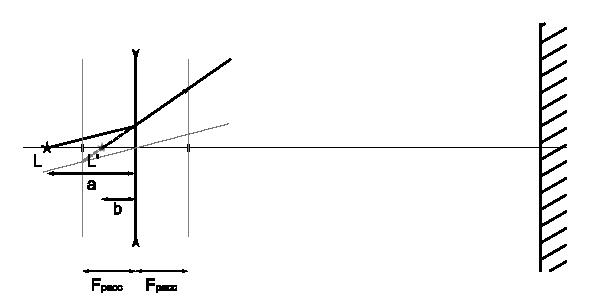
\includegraphics{9kl8-1.pdf}
		    \caption{Изображение, создаваемое рассеивающей линзой}
		    \label{fig:9kl8:rass-step1}
    	} \parbox[b]{\textwidth}{
	    	\centering
		    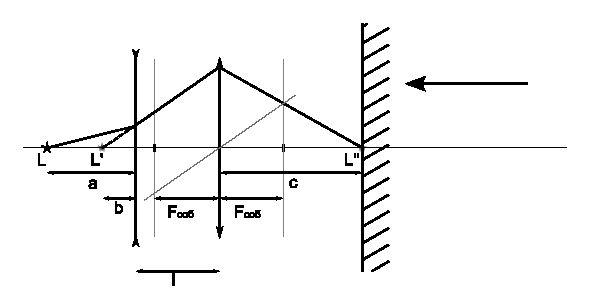
\includegraphics{9kl8-2.pdf}
		    \caption{Конечный вид установки}
		    \label{fig:9kl8:rass-step2}
		}
    \end{figure}
    Используя введенные обозначения для расстояний, запишем формулу тонкой линзы для рассеивающей и собирающей линз:
	\begin{equation}
		\begin{array}{@{}l@{}}
			\frac{1}{F_\text{соб}} = \frac{1}{b+l} + \frac{1}{c} \\
			\frac{1}{F_\text{расс}} = \frac{1}{b} + \frac{1}{a}
		\end{array}
		\Rightarrow
		F_\text{расс} = \frac{c(a F_\text{соб}+al + l F_\text{соб})}{a F_\text{соб} + a l - l F_\text{соб} + a c -c F_\text{соб}}
		\label{eq:9kl8:1}
	\end{equation}
\end{enumerate}
\MesErrors
Будем считать, что абсолютная погрешность измерения всех длин "--- \(\Delta d\). Тогда:
\begin{equation*}
	\varepsilon F_\text{соб} = \Delta d \left( \frac{1}{d_1} + \frac{1}{d_2}+\frac{2}{d_1+d_2} \right)
\end{equation*}
Формулы для вычисления опрделения фокусного расстояния рассеивающей линзы тривиальны и громоздки. Вычисления удобнее проводить по шагам. В формуле~\ref{eq:9kl8:1} обозначим часлитель за \(p\), а знаменатель "--- за \(q\). То:
\begin{equation*}
	\begin{array}{@{}l@{}}
		\Delta p = \Delta d \left( aF_\text{соб}+al-lF_\text{соб}+cF_\text{соб}+cl+ca+cF_\text{соб}\right)+\Delta F_\text{соб} \left(ca+cl\right) \\
		\Delta q = \Delta d \left( 3F+2a+c+l\right) + \Delta F \left(a+l+c\right)
	\end{array}
\end{equation*}
тогда погрешность фокусного расстояния:
\begin{equation*}
	\varepsilon F_\text{расс} = \frac{\Delta p}{p}+\frac{\Delta q}{q}
\end{equation*}
\SchoolBase
\begin{itemize}
    \item Геометрическая оптика. Тонкие линзы, построение изображений.
\end{itemize}
\AdditionalQuestions
\begin{itemize}
    \item Какой способ определения фокусного расстояния собирающей линзы более точен из двух, указанных выше?\par
    \Answer Второй, использующий формулу тонкой линзы, поскольку он позволяет усреднить результат по нескольким принципиально различным измерениям для разного положения источника света. Однако если источник света имеет значительные размеры вдоль оптической оси линзы, метод теряет точность, поскольку изображения разных точек источника будут на разном расстоянии от линзы.
\end{itemize}
\AdditionalNotes
Имеет смысл подробно разобрать физический смысла основных понятий геометрической оптики, таких как {\itshape фокус, фокальная плоскость, изображение}. Разобраться, почему если в изображение поставить экран, на экране будет <<как на фотографии>> видно объект.
